\documentclass[12pt]{article}
\usepackage{graphicx} % Required for inserting images


\usepackage{hyperref}
\usepackage{xcolor}

\hypersetup{
  colorlinks=true,
  citecolor=blue,
  linkcolor=red,
  urlcolor=magenta,
  }
  % citebordercolor=false}

\usepackage{float}
\usepackage{url}
\usepackage{tabularx}
\usepackage{amsmath}
\usepackage{amsfonts}
\usepackage{amssymb}
\usepackage{natbib}
\usepackage{xurl}
\usepackage{lineno}
\usepackage{amsthm}
\usepackage{epsfig}
\usepackage[linesnumbered, ruled]{algorithm2e}

\usepackage{ulem}
\newcommand{\stkout}[1]{\ifmmode\text{\sout{\ensuremath{#1}}}\else\sout{#1}\fi}

\usepackage{multirow}
\usepackage{longtable}
\setlength\LTleft{0pt}
\usepackage{tabularx}

\usepackage{graphicx}
\usepackage{xcolor}
\usepackage{float}
\usepackage{url}
% \setlength\LTleft{0pt}
\usepackage{tabularx}
\usepackage{amsmath}
\usepackage{amsfonts}
\usepackage{amssymb}
\usepackage{natbib}
% \bibliographystyle{unsrt}
\bibliographystyle{agu}
% \bibliographystyle{plainnat}

\newcommand\prob{\mathbb{P}}

\usepackage{xurl} %
%
\usepackage{lineno}

\usepackage{soul}
%
%
\usepackage{amsmath}
\usepackage{amssymb}
\usepackage{amsthm}
\usepackage{float}
%
\usepackage{epsfig}
\usepackage[linesnumbered, ruled]{algorithm2e}

\usepackage{natbib}
\usepackage{color}

%
%
%

\usepackage{multirow}
\usepackage{longtable}
\setlength\LTleft{0pt}
\usepackage{tabularx}
%
\clearpage{}%


\newcommand{\xh}[1]{\textcolor{orange}{\textbf{(xh:)} #1}}

\newcommand{\aj}[1]{\textcolor{magenta}{\textbf{(aj:)} #1}}

%
\newcommand{\resp}[1]{\textcolor{red}{\textbf{Response: } #1}}
\newcommand{\respc}[1]{\textcolor{red}{#1}}


%
\renewcommand{\[}{\left[}
\renewcommand{\]}{\right]}
\renewcommand{\(}{\left(}
\renewcommand{\)}{\right)}

%
\newcommand{\dd}[2]{\frac{d #1}{d #2}}
\newcommand{\ddt}[1]{\frac{d #1}{d t}}
\newcommand{\ddd}[2]{\frac{d^2 #1}{d #2^2}}
\newcommand{\dddt}[1]{\frac{d^2 #1}{d t^2}}
\newcommand{\pp}[2]{\frac{\partial #1}{\partial #2}}
\newcommand{\ppp}[2]{\frac{\partial^2 #1}{\partial #2^2}}
\newcommand{\pppp}[2]{\frac{\partial^3 #1}{\partial #2^3}}
\newcommand{\ppppp}[2]{\frac{\partial^4 #1}{\partial #2^4}}

\newcommand{\adj}[1]{#1^{*}}
\newcommand{\abs}[1]{\left|#1\right|}
\newcommand{\divergence}[1]{\nabla \cdot #1}
\newcommand{\enorm}[1]{\vvvert #1 \vvvert}
\newcommand{\grad}[1]{\nabla #1}
\newcommand{\laplace}[1]{\nabla^2 #1}
\newcommand{\norm}[2]{\left\|\, #1 \,\right\|_{#2}}
\newcommand{\order}[1]{\mathcal{O}\(#1\)}
\newcommand{\supp}{\mathop{\mathrm{supp}}}
\newcommand{\vvvert}{|\kern-1pt|\kern-1pt|}

\newcommand{\eq}[1]{\mathop{\,{\buildrel #1 \over =}\,}}
\newcommand{\ap}[1]{\mathop{\,{\buildrel #1 \over \approx}\,}}

%

%
\newcommand{\hg}{\hat{g}}
\newcommand{\hh}{\hat{h}}
\newcommand{\hi}{\hat{i}}
\newcommand{\hj}{\hat{j}}
\newcommand{\hk}{\hat{k}}
\newcommand{\hm}{\hat{m}}
\newcommand{\hn}{\hat{n}}
\newcommand{\hs}{\hat{s}}
\newcommand{\hu}{\hat{u}}
\newcommand{\hv}{\hat{v}}
\newcommand{\hx}{\hat{x}}

\newcommand{\hA}{\hat{A}}
\newcommand{\hC}{\hat{C}}
\newcommand{\hI}{\hat{I}}
\newcommand{\hJ}{\hat{J}}
\newcommand{\hN}{\hat{N}}
\newcommand{\hT}{\hat{T}}
\newcommand{\hU}{\hat{U}}

\newcommand{\hbf}{\boldsymbol{\hat{f}}}
\newcommand{\hbg}{\boldsymbol{\hat{g}}}
\newcommand{\hsig}{\hat{\sigma}}

%
\newcommand{\barg}{\bar{g}}
\newcommand{\barh}{\bar{h}}
\newcommand{\barm}{\bar{m}}
\newcommand{\barv}{\bar{v}}
\newcommand{\barw}{\bar{w}}
\newcommand{\barx}{\bar{x}}
\newcommand{\bary}{\bar{y}}

\newcommand{\barB}{\bar{B}}
\newcommand{\barC}{\bar{C}}
\newcommand{\barH}{\bar{H}}
\newcommand{\barJ}{\bar{J}}
\newcommand{\barN}{\bar{N}}
\newcommand{\barR}{\bar{R}}

\newcommand{\barmu}{\bar{\mu}}

%
\newcommand{\tf}{\tilde{f}}
\newcommand{\thh}{\tilde{h}}

\newcommand{\tA}{\tilde{A}}
\newcommand{\tg}{\tilde{g}}
\newcommand{\tH}{\tilde{H}}
\newcommand{\tJ}{\tilde{J}}
\newcommand{\tQ}{\tilde{Q}}
\newcommand{\tT}{\tilde{T}}

\newcommand{\tmu}{\tilde{\mu}}
\newcommand{\ttheta}{\tilde{\theta}}
\newcommand{\txi}{\tilde{\xi}}

\newcommand{\tTheta}{\tilde{\Theta}}
\newcommand{\tXi}{\tilde{\Xi}}

%
\newcommand{\mb}[1]{\mathbf{#1}}
\newcommand{\sbf}[1]{\boldsymbol{#1}}

\newcommand{\bb}{\textbf{b}}
\newcommand{\bd}{\textbf{d}}
\newcommand{\bee}{\textbf{e}}
\newcommand{\bff}{\textbf{f}}
\newcommand{\bh}{\textbf{h}}
\newcommand{\bg}{\textbf{g}}
\newcommand{\bk}{\textbf{k}}
\newcommand{\bii}{\textbf{i}}
\newcommand{\bj}{\textbf{j}}
\newcommand{\bl}{\textbf{l}}
\newcommand{\bn}{\textbf{n}}
\newcommand{\bp}{\textbf{p}}
\newcommand{\br}{\textbf{r}}
\newcommand{\bs}{\textbf{s}}
\newcommand{\bt}{\textbf{t}}
\newcommand{\bu}{\textbf{u}}
\newcommand{\bv}{\textbf{v}}
\newcommand{\bw}{\textbf{w}}
\newcommand{\bx}{\textbf{x}}
\newcommand{\by}{\textbf{y}}

\newcommand{\bA}{\mathbf{A}}
\newcommand{\bC}{\mathbf{C}}
\newcommand{\bE}{\mathbf{E}}
\newcommand{\bF}{\mathbf{F}}
\newcommand{\bG}{\mathbf{G}}
\newcommand{\bI}{\mathbf{I}}
\newcommand{\bK}{\mathbf{K}}
\newcommand{\bN}{\mathbf{N}}
\newcommand{\bQ}{\mathbf{Q}}
\newcommand{\bR}{\mathbf{R}}
\newcommand{\bT}{\mathbf{T}}
\newcommand{\bU}{\mathbf{U}}
\newcommand{\bV}{\mathbf{V}}
\newcommand{\bY}{\mathbf{Y}}

\newcommand{\balpha}{\boldsymbol{\alpha}}
\newcommand{\bbeta}{\boldsymbol{\beta}}
\newcommand{\bepsilon}{\boldsymbol{\epsilon}}
\newcommand{\bhsig}{\boldsymbol{\hsig}}
\newcommand{\bpsi}{\boldsymbol{\psi}}
\newcommand{\bsig}{\boldsymbol{\sigma}}
\newcommand{\btau}{\boldsymbol{\tau}}
\newcommand{\bmu}{\boldsymbol{\mu}}
\newcommand{\btheta}{\boldsymbol{\theta}}
\newcommand{\bphi}{\boldsymbol{\phi}}
\newcommand{\bxi}{\boldsymbol{\xi}}

\newcommand{\bDelta}{\boldsymbol{\Delta}}
\newcommand{\bTheta}{\boldsymbol{\Theta}}
\newcommand{\bXi}{\boldsymbol{\Xi}}
\newcommand{\bOmega}{\boldsymbol{\Omega}}
\newcommand{\bSigma}{\boldsymbol{\Sigma}}

%
\newcommand{\EE}{\mathbb{E}}
\newcommand{\II}{\mathbb{I}}
\newcommand{\NN}{\mathbb{N}}
\newcommand{\QQ}{\mathbb{Q}}
\newcommand{\PP}{\mathbb{P}}
\newcommand{\RR}{\mathbb{R}}

%
\newcommand{\vt}{\vec{t}}
\newcommand{\vu}{\vec{u}}
\newcommand{\vv}{\vec{v}}
\newcommand{\vx}{\vec{x}}

\newcommand{\vV}{\vec{V}}

\newcommand{\vo}{\vec{\omega}}

%
\newcommand{\dotk}{\dot{k}}
\newcommand{\dotm}{\dot{m}}
\newcommand{\dotx}{\dot{x}}

\newcommand{\dotomega}{\dot{\omega}}

%
\newcommand{\CA}{\mathcal{A}}
\newcommand{\CB}{\mathcal{B}}
\newcommand{\CD}{\mathcal{D}}
\newcommand{\CE}{\mathcal{E}}
\newcommand{\CF}{\mathcal{F}}
\newcommand{\CH}{\mathcal{H}}
\newcommand{\CJ}{\mathcal{J}}
\newcommand{\CK}{\mathcal{K}}
\newcommand{\CL}{\mathcal{L}}
\newcommand{\CM}{\mathcal{M}}
\newcommand{\CN}{\mathcal{N}}
\newcommand{\CR}{\mathcal{R}}
\newcommand{\CS}{\mathcal{S}}
\newcommand{\CT}{\mathcal{T}}
\newcommand{\CU}{\mathcal{U}}
\newcommand{\CV}{\mathcal{V}}
\newcommand{\CW}{\mathcal{W}}
\newcommand{\CX}{\mathcal{X}}
\newcommand{\CY}{\mathcal{Y}}

\newcommand{\CbarJ}{\bar{\mathcal{J}}}
\newcommand{\CbarL}{\bar{\mathcal{L}}}
\newcommand{\CbarR}{\bar{\mathcal{R}}}

%
\newcommand{\du}{\delta{u}}

\newcommand{\dbeta}{\delta{\beta}}
\newcommand{\dxi}{\delta{\xi}}
\newcommand{\deta}{\delta{\eta}}
\newcommand{\drho}{\delta{\rho}}
\newcommand{\dtau}{\delta{\tau}}

\newcommand{\dbu}{\delta{\boldsymbol{u}}}
\newcommand{\dbp}{\delta{\boldsymbol{p}}}
\newcommand{\dbx}{\delta{\boldsymbol{x}}}

\newcommand{\Dx}{\Delta{x}}
\newcommand{\Dy}{\Delta{y}}
\newcommand{\Dt}{\Delta{t}}

%
\newcommand{\myblue}[1]{{\color[rgb]{0,0,0.65} #1}}
\newcommand{\mygreen}[1]{{\color[rgb]{0,.65,0} #1}}
\newcommand{\mywhite}[1]{{\color[rgb]{1.0,1.0,1.0} #1}}
\newcommand{\myred}[1]{{\color[rgb]{0.65,0.0,0.0} #1}}
\newcommand{\myblack}[1]{{\color[rgb]{0.0,0.0,0.0} #1}}
\newcommand{\mygrey}[1]{{\color[rgb]{0.6,0.6,0.6} #1}}

%
% \newcommand{\coo}{CO$_2$}
% \newcommand{\hho}{H$_2$O}
% \newcommand{\oo}{O$_2$}
% \newcommand{\nn}{N$_2$}
% \newcommand{\mwe}{MW$_e$}
% \newcommand{\nox}{NO$_{\textrm{x}}$}
% \newcommand{\cooe}{CO$_{2e}$}
% \newcommand{\nno}{N$_2$O}
% \newcommand{\noo}{NO$_2$ }
% \newcommand{\chhhh}{CH$_4$ }
% \newcommand{\hhoo}{H$_2$O$_2$}
% \newcommand{\hhoor}{H$_2$-O$_2$}
%
\newcommand{\degs}{^\circ}
% \newcommand{\Jpkmol}{\frac{J}{kmol}}
% \newcommand{\JpkmolK}{\frac{J}{kmol K}}
% \newcommand{\Jpkg}{\frac{J}{kg}}
% \newcommand{\JpkgK}{\frac{J}{kg K}}

\newcommand{\ra}{\rightarrow}
\newcommand{\Ra}{\Rightarrow}
\newcommand{\LRa}{\Longrightarrow}
\newcommand{\lra}{\longrightarrow}

\newcommand{\pe}{\,{\scriptstyle +}\!\!=}
\newcommand{\me}{\,{\scriptstyle -}\!\!=}
\newcommand{\Var}{\textrm{Var}}
\newcommand{\Cov}{\textrm{Cov}}
\newcommand{\diag}{\textrm{diag}}

\newcommand{\etal}{\textit{et al.}}

% \newcommand{\dkl}

\def\sgn{\mathop{\rm sgn}}
\newcommand{\argmax}{\operatornamewithlimits{argmax}}
\newcommand{\argmin}{\operatornamewithlimits{argmin}}
\newcommand{\DKL}{D_{\mathrm{KL}}}

\newcommand{\iid}{\stackrel{\textrm{iid}}{\sim}}
\newcommand{\ti}[1]{\textbf{Title: }\textit{{#1}}}

\newcommand{\alf}{Alfv\'{e}n}
\newcommand{\Rs}{R$_{\odot}$}


\usepackage{algorithmic}
% \usepackage{algpseudocode}



\linenumbers

\title{SVGD-style continuous NFs for Bayesian Inference}
\author{Aniket}
\date{\today}

\begin{document}

\maketitle

(many thanks to Thomas Coons for sparking my interest in this topic - this is a very rich area of computational statistics)

\section{Abstract}

(main motivation is to have a solid and reliable way of building BNNs - also maybe needed for BOED surrogate training if we are looking for MCMC alternatives -  we need to understand the theory behind Stein a bit better for that)

(we will review the use of SVGD for Bayesian Inference, the challenges in scaling it up and if ideas from sparse GPs could be applied to make it more usable with many particles)

(another perspective is that of continuous normalizing flows. Can tricks from these e.g. trace estimators help with the computation for many particles? also, is there an elegant and simple way to tie together the framework of continuous time NNs and weight updates as a single augmented system?)

\begin{enumerate}
    \item SVGD review \cite{liu_short_2016,liu_kernelized_2016,liu_stein_2019}

    \item SVGD drawbacks (mode collapse?) and projected SVGD \cite{chen_projected_2020}

    \item Ideas from sparse GP + VI \url{https://gpss.cc/gpss17/slides/gp-approx-new.pdf} and \cite{noack_unifying_2023}. Slightly better: start from the simplest case i.e. \cite{snelson_sparse_2005} and then move on to \cite{titsias_variational_2009,titsias_bayesian_2010}

    \item Accelerated SVGD? SVI for Deep GPs? \cite{hoffman_stochastic_2013}

    \item are there any ideas from structure preserving methods (is HMC structure preserving?) that can be seamlessly incorporated into SVGD? here are structure preserving Gaussian processes as an example: \url{https://arxiv.org/pdf/2102.01606.pdf}
    
    \item (hopefully) success!
\end{enumerate}

\section{Literature}
We motivate our method by first introducing the concepts of Stein discrepancy, Stein gradient descent, learning kernel operators from Gaussian Processes and the scope for introducing more scalable methods for the same. 

GPs are specified by a placing a Gaussian prior on the space of functions $f$ that model the mapping between inputs $X$ and outputs $y$:

$$p(f | X) = \mathcal{N}(0, K_N)$$

Here $K$ is the (parametrized) covariance kernel which expresses some prior notion of smoothness of the underlying function.

The marginal likelihood $p(y | X, \mathcal{D}, \theta)$ is used to train the GP and learn the hyperparameters. The posterior predictive distribution uses standard formulas for update of the mean and covariance of the prior GP, and is generally prohibitive for vanilla GPs because of the $O(N^3)$ cost of the covariance matrix.

\subsection{Sparse GPs}

\citep{snelson_sparse_2005} To fit a sparse GP, we consider a pseudo-dataset $\bar{\mathcal{D}} = \{(\bar{X}, \bar{f})_m\}_{m=1}^{M}$, with $M<N$ Since the targets are not real observations, they are denoted by $\bar{f}$ instead of $\bar{y}$ and set equal to latent function values.

We have to determine the following:

\begin{enumerate}
    \item Posterior distribution over pseudo-targets $\bar{f}$

    \item Predictive distribution for new $x_{\ast}$

    \item Marginal likelihood expression to find pseudo-input locations!
\end{enumerate}

\subsection{SVGD Algorithm}
Most of the math for SVGD comes from \cite{liu_short_2016,liu_kernelized_2016}.

Consider set of initial particles $\{x_i^0\}_{i=1}^n$ and target density $p(x)$. Then for $l$ update steps, the following transports points from initial distribution to target distribution $p(x)$ (or its approximation $q(x)$)

$$x_i^{l+1} \leftarrow x_i^{l} + \epsilon \frac{1}{n}\sum_{i=1}^{n}\left[k(x_j^l, x) \nabla_{x_j^l}(p(x_j^l)) + \nabla_{x_j^l}k(x_j^l, x)\right]$$

% \begin{algorithm}
% \caption{SVGD from \cite{liu_kernelized_2016}}\label{alg: svgd_vanilla}
% \begin{algorithmic}
% \KwData{$p(x)$}

% \For{\texttt{blah}}
% \STATE $i\gets 10$
% \IF {$i\geq 5$} 
%   \STATE $i\gets i-1$
% \ELSE
%   \IF {$i\leq 3$}
%     \STATE $i\gets i+2$
%   \ENDIF
% \ENDIF

% \end{algorithmic}
% \end{algorithm}

\subsection{Projected SVGD}
\citep{chen_projected_2020} Projected SVGD finds a low-dimensional subspace for projecting $x$ and performs SVGD on a lower dimensional $x$ to avoid the kernel function becoming degenerate for large $d$. This feels like it solves the major problems of SVGD already, but we are probably coming at it from a different angle i.e. just the steps and approximations of the original algorithm and if there are any generalizations or improvements to be pursued there.

\section{Methodology}

Let's start by asking the following questions:
\begin{enumerate}
    \item What kinds of kernels does SVGD hold for? What alternatives exist to avoid degeneracy? The original paper still claims that a lot of the problematic parts of large $n$ can be easily bypassed.

    \item Is there a meaningful connection between determination of pseudo-inputs for sparse GPs and GD style updates? How do we find pseudo-inputs for the SVGD case? \textcolor{red}{remember that this is most likely a fruitless exercise, these ideas are defined for very different applications: entirely non-parametric methods vs NNs where people look for nice ways to combine optimization over NN parameters (data-fitting) with posterior updates for the weights.}

    \textcolor{red}{We either need stand-alone kernel approximations - which don't involve learning inducing points, or a clever way to learn inducing point locations}

    \begin{enumerate}
        \item Initialize inducing points

        \item (some update step for transporting inducing points)

        \item (some correction step for moving them around so they represent the original dataset)
    \end{enumerate}

    \item What are the precise connections between SVGD and flow-based models like CNFs? Can we combine neural network weight updates in a flow-based model with posterior computations?

    \textcolor{blue}{The simplest thing we can actually try, funnily enough, is just replacing $p(.)$ by some MLP and / or a richer kernel representation for $k$ - the points being that}
    
    \begin{enumerate}
        \item we can get rid of the variational family and consider a more general case - if there is a strong case for the quality of posterior learnt by VI

        \item Right now a lot of the methodology here feels like a bunch of tricks to learn the kernel hyperparameters - but surely there is a rigorous way to actually learn these, or a more general and flexible form of Stein that accomodates different choices - again, if there are advantages for a different kernel family (how do we show this?) - the theory and literature on spectral delta kernels makes it clear that there are problems where composing kernels or learning an arbitrary stationary kernel is beneficial. 
    \end{enumerate}

    \item SVGD for Monte-Carlo integration (in combination with level-set methods)
\end{enumerate}

% Here is the original algorithm for performing SVGD (assume RBF kernel):


% \noindent Here's our approximation.


% \noindent Here's the modified algorithm.

Let's write down some notes for answering question 3 first:

First we remember that the map is usually constructed to be invertible, starting from the data-generating distribution $x$ and mapping to a standard base distribution (e.g. particles from $q_0$) i.e. the flow direction is reversed. The invertibility ensures we can then draw from the base distribution to sample the posterior distribution.

Let $l$ represent the artificial depth variable or the time variable for integration, and $y_i$ some state variable we wish to update then:

$$y_i^l = y_i^0 + \int_0^{l}g_\theta(y_0, l)dl$$

where $g_\theta$ is the MLP for the flow dynamics.

For CNFs the above can be written as:

$$\log p(x) = \log p(x_0) + \int_l^0 -\operatorname{Tr}\left(\frac{\partial f}{\partial x}\right) dl$$

\stkout{The base distribution gets approximated by particles over here as well, so we end up with (for a single step update):}

$$x_i^{l+1} = x_i^{l} + \int_{t_{l + 1}}^{t_l} -\operatorname{Tr}\left(\frac{\partial f}{\partial x}\right) dl$$


and at the final step:

$$x_i^{l} = x_i^{0} + \int_{l}^{0}\operatorname{Tr}\left(\frac{\partial f}{\partial x}\right) dl $$

\textcolor{red}{okay, so the above is definitely wrong. Its not that the base distribution is approximated by particles, rather CNF solves an augmented system where we find the particle that generates a specific $x$ and solve for the instantaneous change of variables formula that maximizes the log-likelihood of $x$ under that transformation.}


\stkout{(doing what's already been done before and probably isn't very remarkable once I think about it a little more, unless I am very mistaken). Let's take a small step back. Before we introduce the kernel function, the original Stein operator based update, when using a variational family $q(x)$ to approximate $p(x)$ reads as:}

% $$x_i^{l+1} = x_i^{l} + \mathbb{E}_{x \sim q}\left[-\operatorname{Tr}(\mathcal{A}_p \phi(x))\right]$$

\begin{equation*}
    x_i^{l+1} = x_i^{l} + \epsilon \mathbf{\phi}_{\hat{\mu}_l^n, p}^{\ast}(x_l^i)
\end{equation*}

the problematic part of the Stein approximation is that of the non-linear velocity field $\phi$ which should maximally decrease KL divergence w.r.t. target distribution. 

Another way to write it is through the operation of a fixed point non-linear map on empirical measure $\hat{\mu}$:

$$\hat{\mu}_{l + 1}^n = \Phi_p (\hat{\mu}_l^n)$$

% or,

% $$x_i^{l+1} = x_i^{l} + \int \left[-\operatorname{Tr}(\mathcal{A}_p \phi(x))\right] q(x) dx$$


\section{General Literature}

\noindent \textbf{Latent Force Models:} Connecting Differential Equations and GP Kernels - see \cite{alvarez09a} for details.

\noindent This assumes latent forcing functions that give rise to the state evolution of the system, and assuming a GP prior on those functions leads to closed form expressions for the output kernel. Then the log-likelihood can be minimized, leading to standard inference based on GP regression.

\noindent \textbf{Sparse Spectrum Kernels:} Based on trigonometric basis functions, Fourier duals - see \cite{lazaro-gredilla_sparse_2010}

Details of Stein's Operator and Applications: See \cite{anastasiou_steins_2023}

\noindent Derivation of SVGD!


\noindent Rewriting the Variational part with a different approximation (\textsc{REINFORCE} vs the reparametrization trick! - see \url{https://stillbreeze.github.io/REINFORCE-vs-Reparameterization-trick/} for details


\noindent Details of amortized Stein for training probabilistic NNs: See \cite{feng_learning_2017}


\noindent \textbf{Particle transport methods} \emph{``Particles may be regarded as Dirac-delta approximations of otherwise continuous measures or densities. However, continuum transport problems differ from true particle-dynamics problems in one important respect $\cdots$ The velocity field that governs the instantaneous motion of the particles depends on local density gradients, not just particle positions.''} - from paper on OT methods for advection-diffusion \cite{fedeli_geometrically-exact_2017}. An example of advection using particle based methods can be found here: \href{https://docs.oceanparcels.org/en/latest/examples/tutorial_analyticaladvection.html}{Lagrangian simulators!} and some more thoughts on this over here: \url{https://math.temple.edu/~seibold/research/meshfree/}

\noindent \textbf{SVGD as Gradient Flow} Stein is a particle-based approximation to an evolutionary PDE of densities or measures...\emph{Empirical measures of SVGD samples weakly converge to the target distribution, $\cdots$ asymptotic behaviour $\cdots$ characterized by a nonlinear Fokker-Planck equation known as Vlasov equation in physics.} \cite{liu_stein_2017}

Our understanding here is still incomplete, mainly w.r.t the following few points:

\begin{enumerate}
    \item Derivation of the gradient flow equation - I am completely lost in the steps there - some trace trick?

    \item Derivation of the gradient step of KL in terms of the kernel and the Fisher score

    \item Minimization of other Stein discrepancies (non-kernelized) (see \cite{anastasiou_steins_2023} for overview)

    \item Theorem 3.3 from \cite{liu_stein_2017}

    \item Fixed point iteration perspective vs differential equation perspective (one is for particles while the other is for densities??)
\end{enumerate}

\begin{figure}[H]
    \centering
    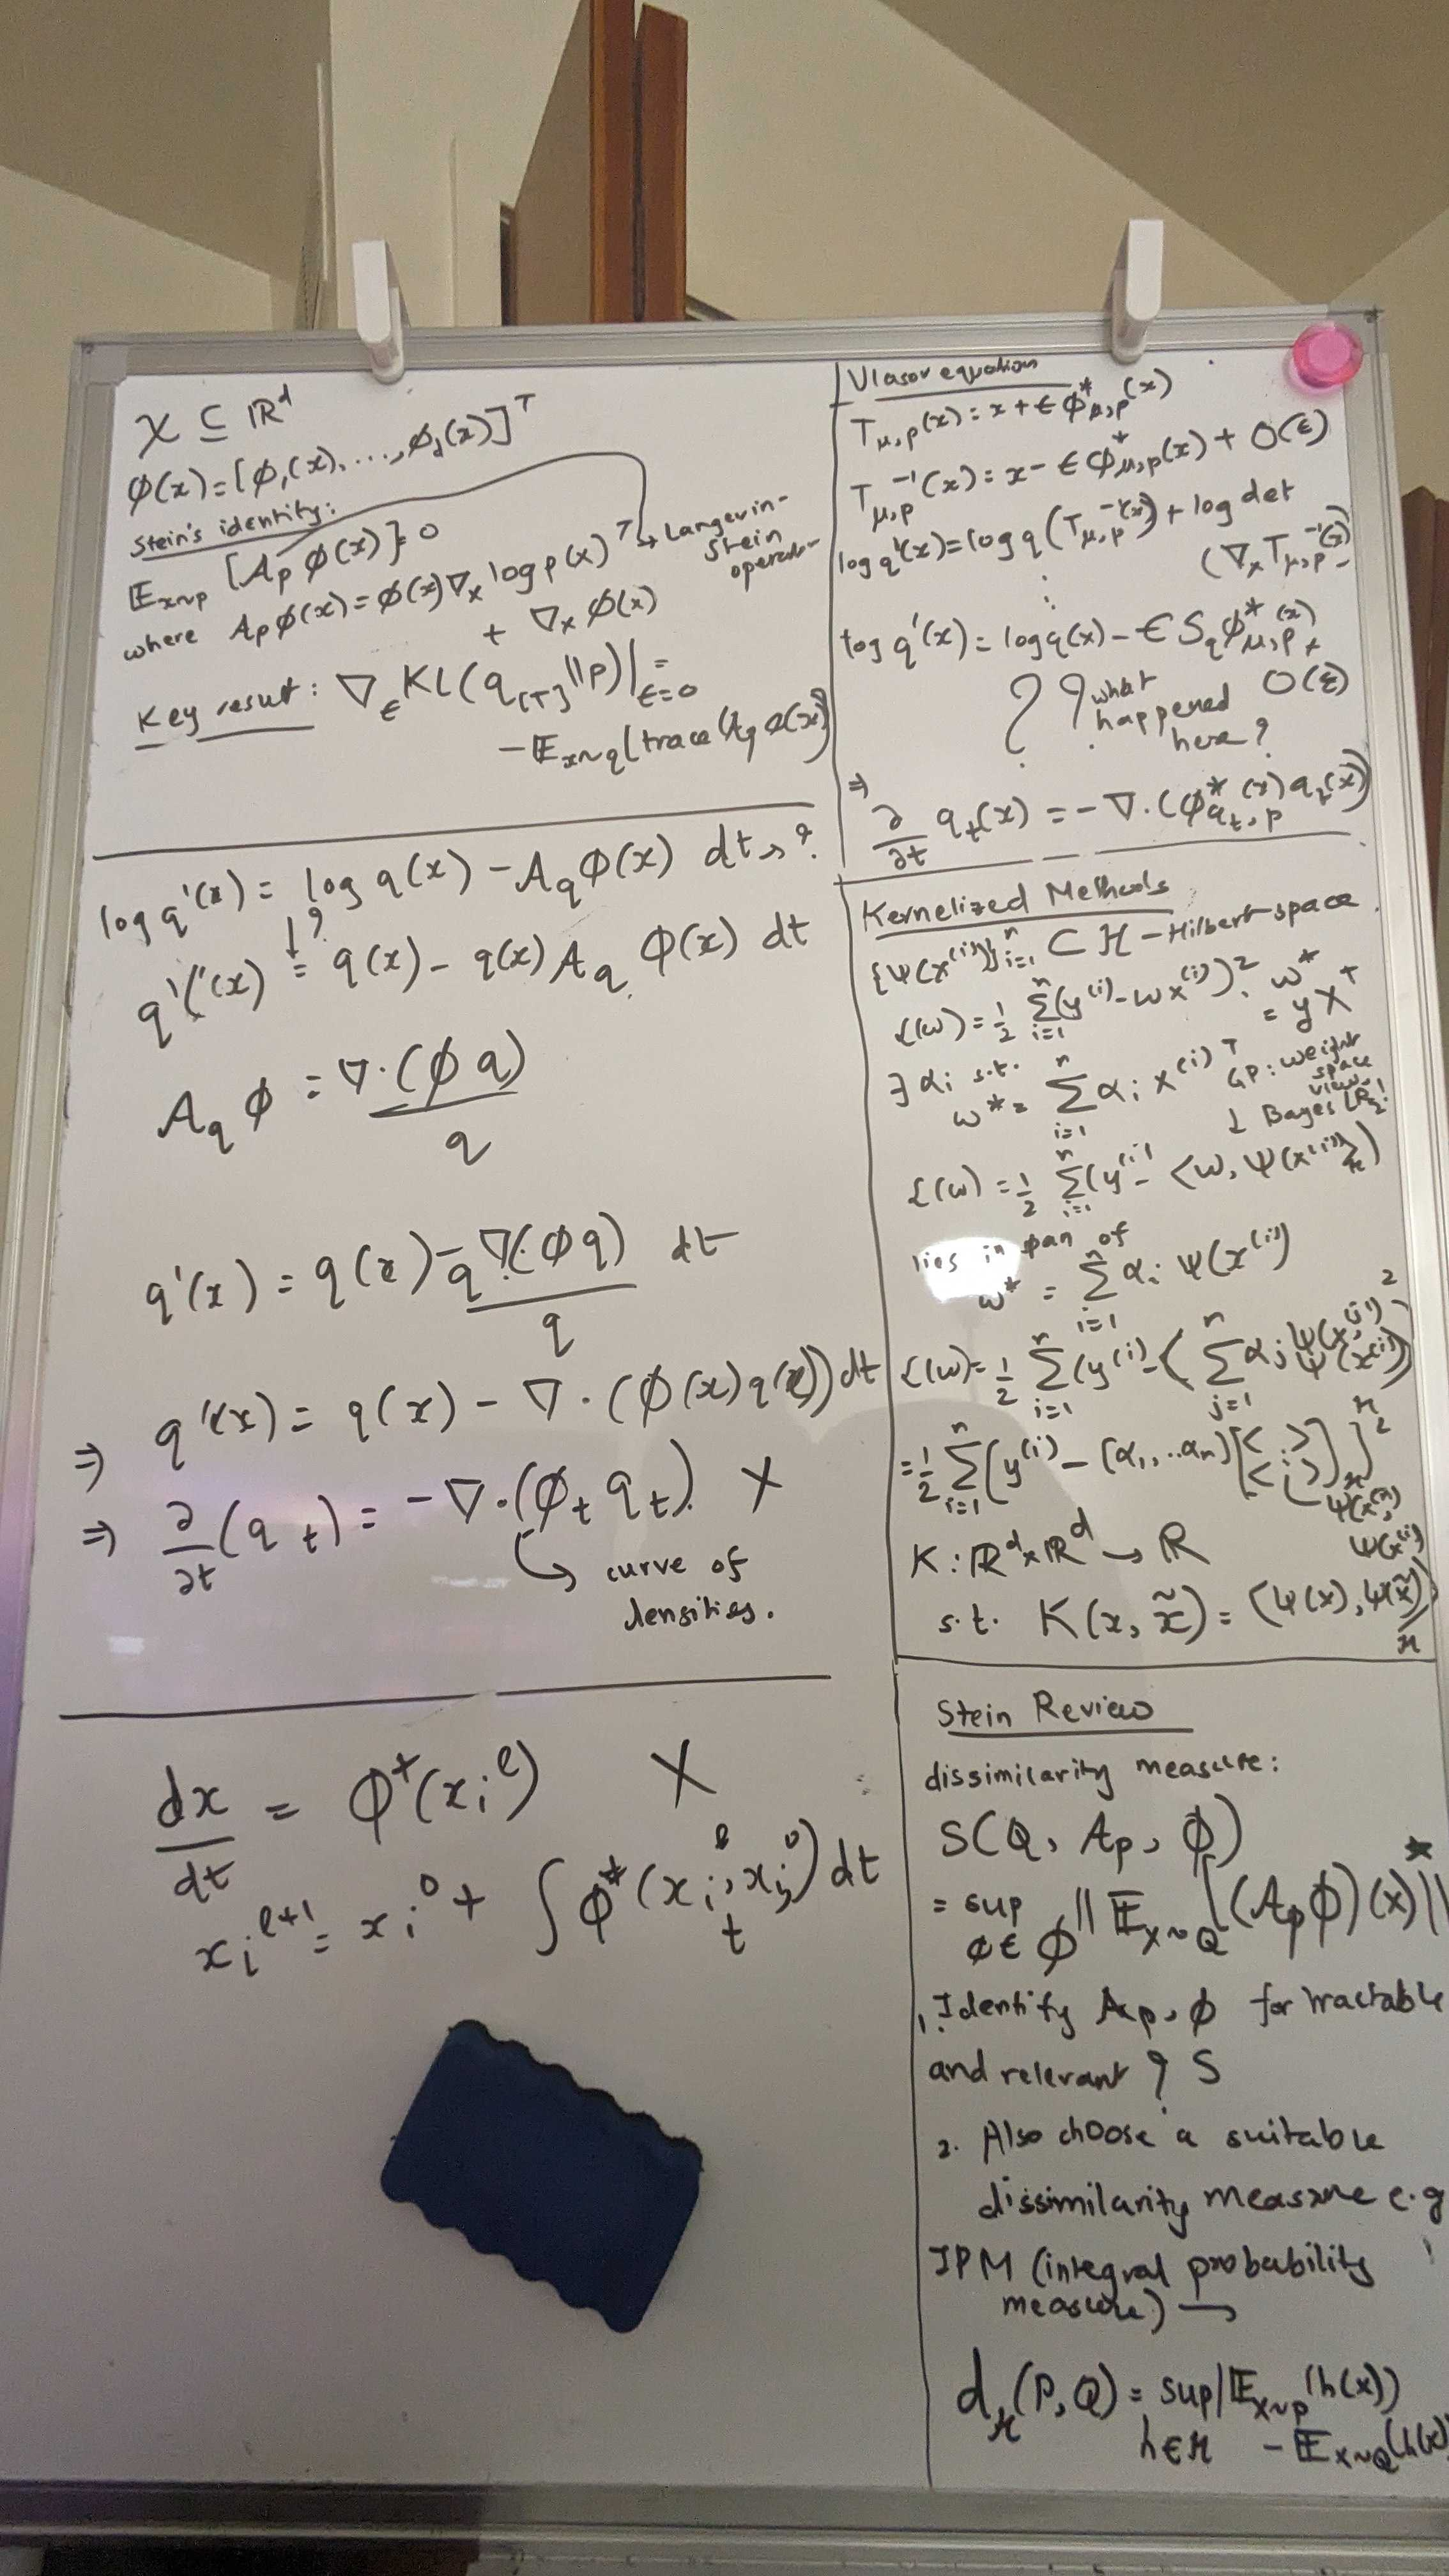
\includegraphics[width=0.6\textwidth]{figures/stein_overview.jpg}
    \caption{My rudimentary understanding of the ideas involved in Stein}
    \label{fig:stein-big-picture}
\end{figure}

Based on the above, however, we can draw up a very rough action plan!

\begin{enumerate}
    \item \stkout{How many particles are too many? i.e. when does the kernel approximation really break down? Probably need to stress test on some tougher canonical example for this.} How many particles are too little? How costly is it to run more particles? (with all tricks related to subsampling etc.)? Stress test on a tougher canonical example. Definitely , pSVGD could also be an interesting use case (numerical stability of active subspace eigenvectors?? - see \cite{hauth_advances_2024} for details.)

    \item Start with the augmented CNF \cite{grathwohl_ffjord_2018}:
    $$\underbrace{\begin{bmatrix}\mathbf{z}_0\\\log p(\mathbf{x})-\log p_{z_0}(\mathbf{z}_0)\end{bmatrix}}_{\text{solutions}}=\underbrace{\int_{t_1}^{t_0}\begin{bmatrix}f(\mathbf{z}(t),t;\theta)\\-\operatorname{Tr}\left(\frac{\partial f}{\partial\mathbf{z}(t)}\right)\end{bmatrix}dt}_{\text{dynamics}},\quad\underbrace{\begin{bmatrix}\mathbf{z}(t_1)\\\log p(\mathbf{x})-\log p(\mathbf{z}(t_1))\end{bmatrix}=\begin{bmatrix}\mathbf{x}\\0\end{bmatrix}}_{\text{initial values}}$$

    and replace $f$ by the Stein update (so we need to find the expression with the kernel, and also get its trace!) - if we are not doing something silly here.

    Then we can run a few comparisons right off the bat with CNFs: Number of function evaluations needed in forward and backward pass, plots of learnt dynamics (are they regularized out of the box?!) and also try experiments with a bunch of kernels.

    To be clear, we also need to investigate some claims in greater detail, notably performance improvements of CNFs over NFs, 
    % what freedom it allows in terms of choice of $f$ and trying to find more robust links between the OT-based regularization and any `implicit' regularization in Stein's method. The motivation is also not completely clear, and we should clarify how it fits into the broader aims of the thesis too.

    \textcolor{red}{One key advantage may be that once the change of variables formula has been simplified to use the trace, unbiased estimators of the trace can be deployed, resulting in a free-form Jacobian.}

    \textcolor{red}{What then about the form of $f$?} One idea is that $f = \grad_x \log p(x) \phi(x)^T + \grad_x \phi(x)$ where $\phi$ can now be replaced by any suitable choice of kernel.

    

    \item More theoretical stuff, quality of posterior compared to other methods, more (faraway) thoughts on kernel approximations.
\end{enumerate}



\section{Results}

\section{Conclusions}


\bibliography{local,references}

\end{document}

